\documentclass[a4paper,12pt]{article}
\usepackage[utf8x]{inputenc}
\usepackage{fullpage}
\usepackage[polish]{babel}
\usepackage{polski}
\usepackage{listings}
\usepackage{amsfonts}
\usepackage{amsmath}
\usepackage{graphicx}
\usepackage{float}
\usepackage{subfig}
\lstset{language=matlab}

\begin{document}
\title{Wyostrzanie obrazu - projekt PSZT}
\date{semestr 13L}
\author{Paweł Stiasny, Michał Baranowski, Michał Świętochowski}
\maketitle

%%%%%%%%%%%%%%%%%%%%%%%%%%%%%%%%%%%%%%%%%%%%%%%%%%%%%%%%%%%%%%%%%%%%%%%%%%%%%%%
\section{Decyzje projektowe}
Tematem zadania było zaimplementowanie algorytmu wyostrzania obrazu
z użyciem logiki rozmytej.

Wykorzystany przez nas algorytm działa trójetapowo:
\begin{enumerate}
	\item Traktując każdy piksel obrazu jako rozmyty singleton, modyfikuje 
		jego wartość przynależności na podstawie funkcji wzmacniającej kontrast
		\[
			\mu' = \mbox{INT}(\mu) =
			\begin{cases}
				2 \mu^2 & \mbox{dla } 0 \leq \mu \leq 0.5 \\
				1 - 2(1 - \mu)^2  & \mbox{dla } 0.5 \leq \mu \leq 1 \\
			\end{cases}
		\]
	\item Wygładza obraz zastępując wartość przynależności każdego piksela
		warością uśrednioną jego sąsiadów, tj. dokonuje splotu obrazu
		z macierzą
		\[
			\begin{bmatrix}
				0 & \frac 1 4 & 0 \\
				\frac 1 4 & 0 & \frac 1 4 \\
				0 & \frac 1 4 & 0
			\end{bmatrix}
		\]
	\item Powtarza operację z punktu 1 na uzyskanym obrazie
\end{enumerate}

Do implementacji zadania użyliśmy języka Python, wykorzystując popularną
bibliotekę wspomagającą obliczenia macierzowe: numpy.  Dodatkowo do obsługi
obrazów posłużyła biblioteka scikit.

%%%%%%%%%%%%%%%%%%%%%%%%%%%%%%%%%%%%%%%%%%%%%%%%%%%%%%%%%%%%%%%%%%%%%%%%%%%%%%%
\section{Uruchomienie programu}
W skład projektu wchodzą dwa skrypty wykonywalne: improc.py oraz test.py.
Pierwszy z nich jako argumenty pobiera ścieżkę do pliku obrazu wejściowego
oraz wyjściowego.  Drugi w trybie wsadowym uruchamia algorytm dla wszystkich
obrazów w katalogu testin projektu i umieszcza rezultaty w katalogu testout.

Do uruchomienia konieczne jest spełnienie zależności programu.  W systemie
musi być zainstalowany interpreter Pythona w wersji 2.7 oraz następujące
biblioteki:
\begin{itemize}
	\item numpy
	\item scikit
	\item PIL
\end{itemize}

%%%%%%%%%%%%%%%%%%%%%%%%%%%%%%%%%%%%%%%%%%%%%%%%%%%%%%%%%%%%%%%%%%%%%%%%%%%%%%%
\section{Struktura programu}
Program składa się z wymienionych wcześniej skryptów wykonywalnych obsługujących
wczytywanie i zapisywanie obrazów, oraz z modułu fuzzy implementującego
główne funkcje projektu opisane w sekcji 1.  Wszystkie operacje korzystają z
zapisu macierzowego, co pozwala uzyskać zadawalającą efektywość pomimo użycia
interpretowanego środowiska, a jednocześnie wpływa pozytywnie na czytelność
kodu.

%%%%%%%%%%%%%%%%%%%%%%%%%%%%%%%%%%%%%%%%%%%%%%%%%%%%%%%%%%%%%%%%%%%%%%%%%%%%%%%
\section{Rezultaty}
Oto kilka przykładów działania naszego programu:

\includegraphics[scale=0.7]{testin/moon_low_contrast.png}

\includegraphics[scale=0.7]{testout/moon_low_contrast.png}

\includegraphics{testin/czacha.png}
\includegraphics{testout/czacha.png}

Jak widać, udało się uzyskać wyraźną emfazę widocznych na obrazach kształtów,
co jest istotne przy wzrokowej identyfikacji przedmiotów.

%%%%%%%%%%%%%%%%%%%%%%%%%%%%%%%%%%%%%%%%%%%%%%%%%%%%%%%%%%%%%%%%%%%%%%%%%%%%%%%
\section{Bibliografia}
\begin{itemize}
	\item Podstawy Sztucznej Inteligencji -- preskrypt -- Paweł Wawrzyński
	\item Introduction to Fuzzy Logic using MATLAB -- S.N. Sivanandam, S.
		Sumathi and S.N. Deepa
	\item Image Enhancement Based On Fuzzy Logic -- IJCSNS International Journal
		of Computer Science and Network Security, VOL.9 No.10, October 2009 --
		Mr. Harish Kundra, Er. Aashima, Er. Monika Verma
\end{itemize}

\end{document}
